\begin{figure}[h]
    \centering
    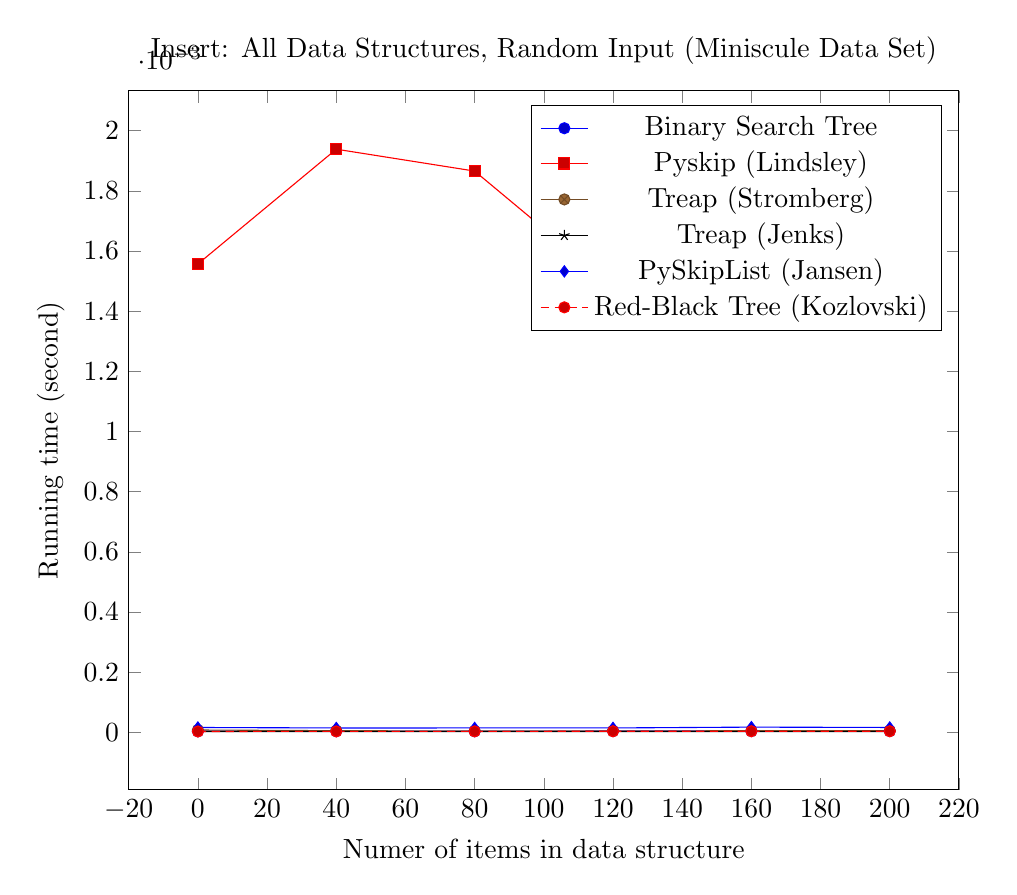
\begin{tikzpicture}
        \begin{axis}[
            xlabel={Numer of items in data structure},
            ylabel={Running time (second)},
            title={Insert: All Data Structures, Random Input (Miniscule Data Set)},
            width=\textwidth
        ]
		\addplot coordinates {
			(0, 3.28281117059348e-06)
			(40, 3.6141040410192505e-06)
			(80, 3.4333988389673165e-06)
			(120, 4.276689781873566e-06)
			(160, 4.126102113496955e-06)
			(200, 4.0959845798216324e-06)
		};
		\addplot coordinates {
			(0, 0.0015570764910061512)
			(40, 0.001938665642670523)
			(80, 0.001865901681311316)
			(120, 0.0014826259477611348)
			(160, 0.001903608833472631)
			(200, 0.0017520272864855134)
		};
		\addplot coordinates {
			(0, 7.6197360198149156e-06)
			(40, 5.300685926823423e-06)
			(80, 4.336924849224211e-06)
			(120, 4.397159916580406e-06)
			(160, 5.2103333258113335e-06)
			(200, 5.2404508594783294e-06)
		};
		\addplot coordinates {
			(0, 2.6804604970953604e-06)
			(40, 2.4696377613597774e-06)
			(80, 2.258815025635297e-06)
			(120, 2.288932559313395e-06)
			(160, 2.108227357267012e-06)
			(200, 2.6202254297391647e-06)
		};
		\addplot coordinates {
			(0, 1.593217531415947e-05)
			(40, 1.4396181096731909e-05)
			(80, 1.4456416164077002e-05)
			(120, 1.4456416164077002e-05)
			(160, 1.716699419485046e-05)
			(200, 1.6022527915182662e-05)
		};
		\addplot coordinates {
			(0, 2.710578030762356e-06)
			(40, 2.9515183001649346e-06)
			(80, 3.102105968544322e-06)
			(120, 3.433398838970092e-06)
			(160, 3.493633906326288e-06)
			(200, 3.4936339063151855e-06)
		};
        \legend{Binary Search Tree, Pyskip (Lindsley), Treap (Stromberg), Treap (Jenks), PySkipList (Jansen), Red-Black Tree (Kozlovski)}
        \end{axis}
    \end{tikzpicture}
    \caption{Average of 10 operations, benchmarked every 40, starting at 0.}
\end{figure}